% -*- mode:LaTeX; mode:visual-line; mode:flyspell; fill-column:75 -*-
\section{Introduction}
\label{secIntroduction}

Enabling robots to understand natural language would provide an intuitive interface between lay users and complex robots.
Prior work on enabling robots to understand language has addressed diverse tasks such as following route directions through indoor and outdoor environments~\cite{macmahon06, kollar10, matuszek12a, duvallet13, boularias15}, mobile manipulation~\cite{tellex11, howard14a}, or building semantically-annotated maps of the environment~\cite{walter13}.

These approaches typically map language to robot plans or high-level symbolic robot languages, and as they are focused solely on high-level reasoning they assume that a controller exists that can adequately execute the desired actions.
Hence, natural language has been used mainly as a means of communicating final or intermediate task goals to the robot (e.g., route directions), but not in specifying \emph{how} to reach those goals.
Our work addresses this gap by leveraging the expressiveness of language and the power of Dynamical Systems-based motion generation.
This could enable language-based control of robots performing complex tasks that require reasoning at the trajectory level such as fine manipulation tasks, variable-impedance tasks, or tasks that .

Dynamical Systems (DS) based approaches have emerged as an extremely effective means of representing trajectories, and provides several key benefits:
they are robust to perturbations of the robot,
they are robust to perturbations in the environment,
and they generalize well across entire families of trajectories.
Such DS models are usually tailored to specific tasks via learning from demonstration or reinforcement learning~\ref{klas_cite_papers_here}.
Connecting natural language and Dynamical Systems would enable users to communication both \emph{what} to do and \emph{how} to do it in a unified representation.

In this report, we explore NL for online modification of DS models belonging to a recently proposed framework allowing incremental learning in stable DS models \todo[inline]{cite klas's RAS paper}. \todo[inline]{need some sort of example on how the system works from the perspective of the user, e.g. what happens when we say turn left etc.}.
We train a model from human demonstrations of the desired behavior modifications (using kinesthetic teaching), and generalize those to novel states in the world.
During execution, the user can then change the behavior of robot (through the controller) by using the trained natural language commands.



\begin{figure}[t]
  \centering
  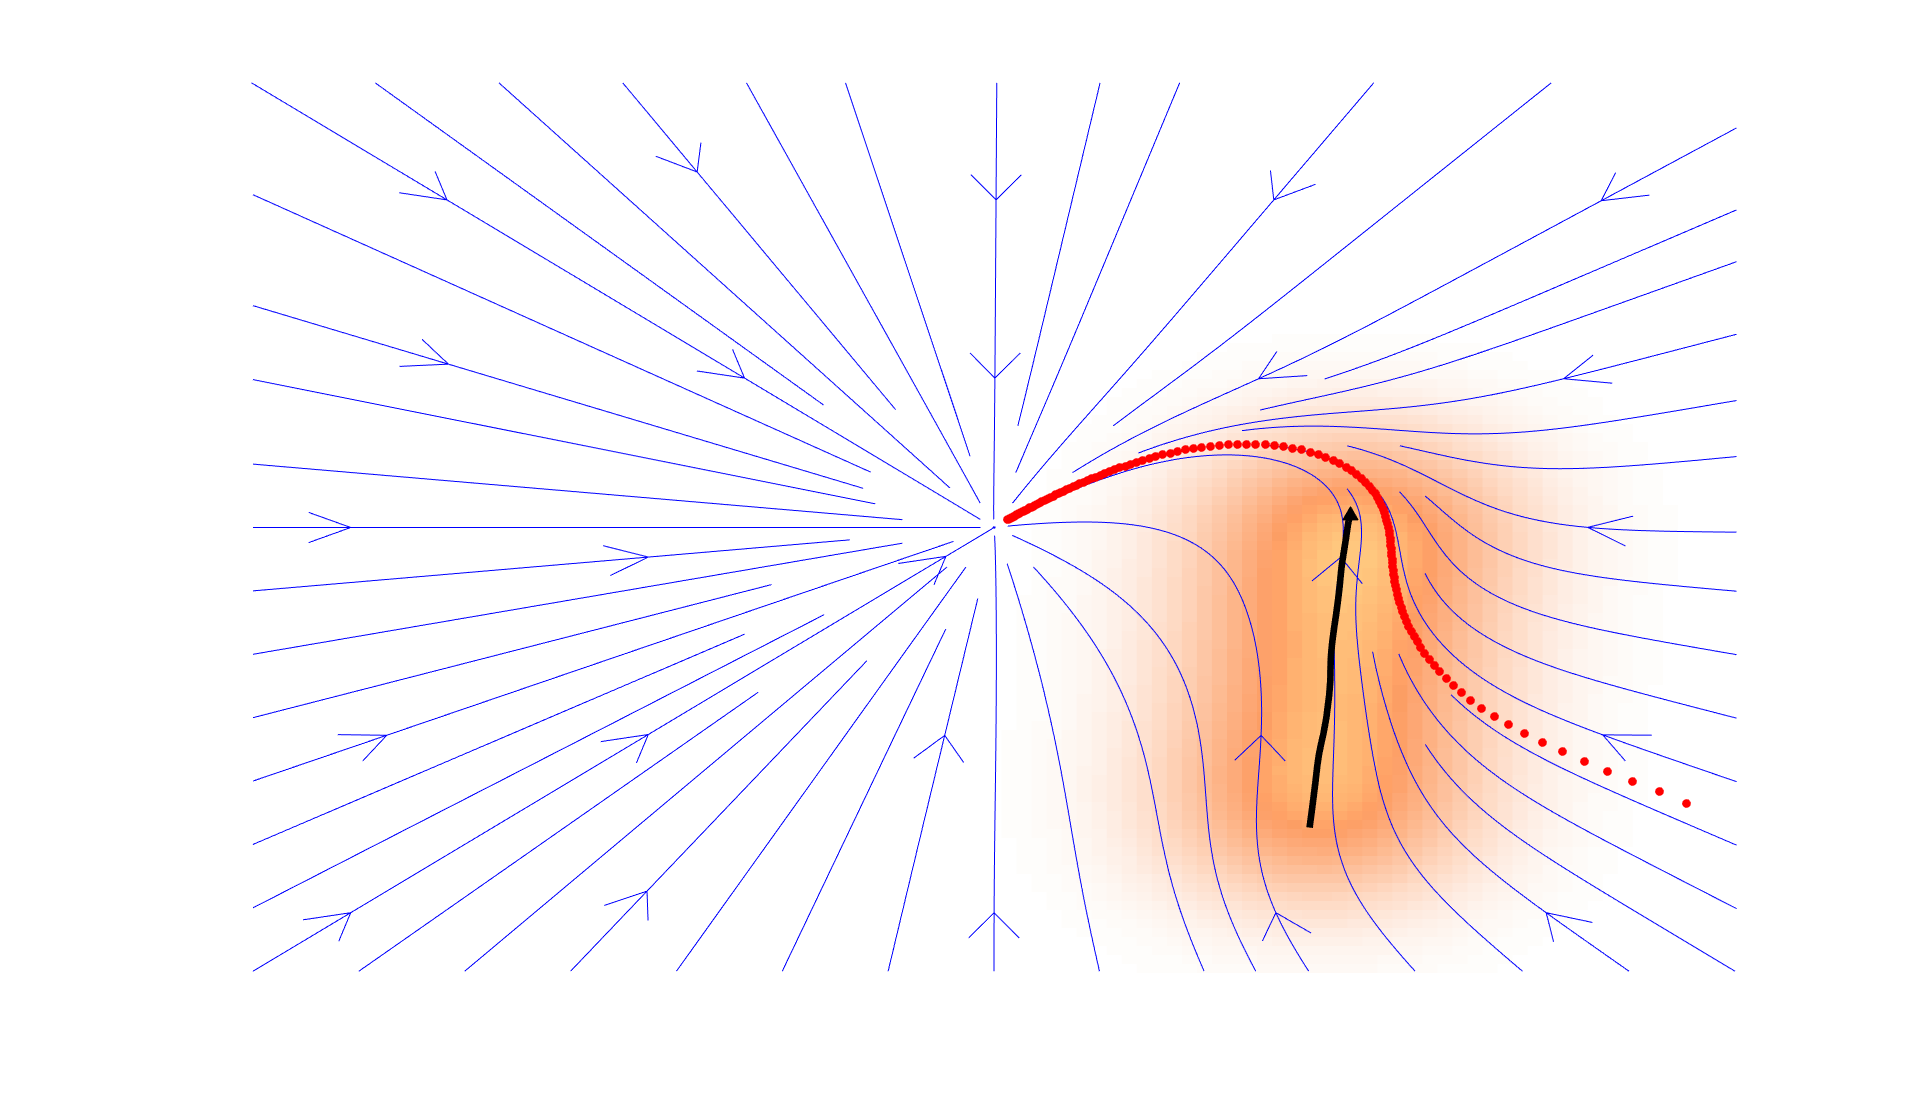
\includegraphics[
    % trim = left bottom right top
    trim = 150mm 50mm 100mm 80mm, clip,
    width = 0.4\textwidth,
  ]{figs/gp_figs/3a-traj1.png}
  \caption{A Modified Dynamical System, representing the controller policy over the entire state space (a 2D plane in this example): at every point the robot follows the gradient until it reaches the attractor.
 In the colored areas, the user has provided a correction to the policy (black arrow), which updates the policy in the same region of state space (re-shaped blue lines),
 resulting in behavior that generalizes to other nearby areas of the state space: for example the red trajectory.
    Our goal is to use natural language to modify a dynamical system, resulting in trajectories that performs the desired behavior.
}
  \label{figProblemSetup}
\end{figure}



% For example, an assistive robot may need to understand how much pressure it should exert when cleaning a patient's skin,
% or a factory robot may need to change how stiffly it should hold a part when cooperatively holding it for a person to assemble,
% or a <> robot may need to know from which direction to approach an object
